\documentclass[a4paper, 12pt]{article}        % General format
%\documentclass[a4paper, 14pt]{extarticle}    % Advanced format

%%%% Charset
\usepackage{cmap}                             % Make PDF files searchable and copyable
\usepackage[utf8x]{inputenc}                  % Accept different input encodings
\usepackage[T2A]{fontenc}                     % Russian font
\usepackage[russian]{babel}                   % Multilingual support (T2A)

%%%% Graphics
\usepackage[dvipsnames]{xcolor}               % Driver-independent color extensions
\usepackage{graphicx}                         % Enhanced support for graphics
\usepackage{wrapfig}                          % Produces figures which text can flow around
\usepackage{float}                            % Improved interface for floating objects

%%%% Graphs
\usepackage{tikz}                             % Creating graphics programmatically
\usetikzlibrary{arrows}                       % Arrows for tikz

%%%% Math
\usepackage{amsmath}                          % American Mathematical Society (AMS) math facilities
\usepackage{amsfonts}                         % fonts from the AMS
\usepackage{amssymb}                          % additional math symbols

%%%% Typography (don't forget about cm-super)
\usepackage{microtype}                        % subliminal refinements towards typographical perfection
\linespread{1.3}                              % line spacing
\usepackage[left=2.5cm, right=1.5cm, top=2.5cm, bottom=2.5cm]{geometry}
\setlength{\parindent}{0pt}                   % we don't want any paragraph indentation
\usepackage{parskip}                          % add distance between paragraphs

%%%% Tables
\usepackage{tabularx}                         % Enhanced tables
\usepackage{multirow}                         % For tabular
\usepackage{hhline}                           % For tabular

%%%% Other
\usepackage{url}                              % Verbatim with URL-sensitive line breaks
\usepackage{fancyvrb}                         % Sophisticated verbatim text
\setcounter{secnumdepth}{5}                   % Turn on subsection numbering

%------------------------------------------------------------------------------
\usepackage{listings}                         % typeset source code listings

% The colors for syntax highlighting.
\definecolor{mygreen}{HTML}{3F7F5F}           % color values Red, Green, Blue
\definecolor{mylilas}{RGB}{170,55,241}

% Code listing settings
\lstset{language=Matlab,%
    %basicstyle=\color{red},
    breaklines    =  true,                    % wrap long lines
    morekeywords  =  {matlab2tikz},           %
    keywordstyle  =  \color{blue},            %
    morekeywords  =  [2]{1},                  %
    keywordstyle  =  [2]{\color{black}},      %
    identifierstyle= \color{black},           %
    stringstyle   =  \color{mylilas},         %
    commentstyle  =  \color{mygreen},         %
    showstringspaces=false,                   % don't mark spaces in strings
    frame         =  tblr                     % draw a frame at all sides of the code block
    rulecolor     =  \color{frame},           % frame color
    tabsize       =  2,                       % tab space width
    showstringspaces=false,                   % don't mark spaces in strings
    numbers       =  left,                    %
    numberstyle   =  {\tiny \color{black}},   % size of the numbers
    numbersep     =  9pt,                     % this defines how far the numbers are from the text
    emph          =  [1]{for,end,break},      %
    emphstyle     =  [1]\color{red},          % some words to emphasise
    %emph         =  [2]{word1,word2},        %
    %emphstyle    =  [2]{style},              %
    extendedchars =  true,                    % For the Russian language support
    literate=
        {Ö}{{\"O}}1                    {Ä}{{\"A}}1                    {Ü}{{\"U}}1
        {ß}{{\ss}}1                    {ü}{{\"u}}1                    {ä}{{\"a}}1
        {ö}{{\"o}}1                    {~}{{\textasciitilde}}1        {а}{{\selectfont\char224}}1
        {б}{{\selectfont\char225}}1    {в}{{\selectfont\char226}}1    {г}{{\selectfont\char227}}1
        {д}{{\selectfont\char228}}1    {е}{{\selectfont\char229}}1    {ё}{{\"e}}1
        {ж}{{\selectfont\char230}}1    {з}{{\selectfont\char231}}1    {и}{{\selectfont\char232}}1
        {й}{{\selectfont\char233}}1    {к}{{\selectfont\char234}}1    {л}{{\selectfont\char235}}1
        {м}{{\selectfont\char236}}1    {н}{{\selectfont\char237}}1    {о}{{\selectfont\char238}}1
        {п}{{\selectfont\char239}}1    {р}{{\selectfont\char240}}1    {с}{{\selectfont\char241}}1
        {т}{{\selectfont\char242}}1    {у}{{\selectfont\char243}}1    {ф}{{\selectfont\char244}}1
        {х}{{\selectfont\char245}}1    {ц}{{\selectfont\char246}}1    {ч}{{\selectfont\char247}}1
        {ш}{{\selectfont\char248}}1    {щ}{{\selectfont\char249}}1    {ъ}{{\selectfont\char250}}1
        {ы}{{\selectfont\char251}}1    {ь}{{\selectfont\char252}}1    {э}{{\selectfont\char253}}1
        {ю}{{\selectfont\char254}}1    {я}{{\selectfont\char255}}1    {А}{{\selectfont\char192}}1
        {Б}{{\selectfont\char193}}1    {В}{{\selectfont\char194}}1    {Г}{{\selectfont\char195}}1
        {Д}{{\selectfont\char196}}1    {Е}{{\selectfont\char197}}1    {Ё}{{\"E}}1
        {Ж}{{\selectfont\char198}}1    {З}{{\selectfont\char199}}1    {И}{{\selectfont\char200}}1
        {Й}{{\selectfont\char201}}1    {К}{{\selectfont\char202}}1    {Л}{{\selectfont\char203}}1
        {М}{{\selectfont\char204}}1    {Н}{{\selectfont\char205}}1    {О}{{\selectfont\char206}}1
        {П}{{\selectfont\char207}}1    {Р}{{\selectfont\char208}}1    {С}{{\selectfont\char209}}1
        {Т}{{\selectfont\char210}}1    {У}{{\selectfont\char211}}1    {Ф}{{\selectfont\char212}}1
        {Х}{{\selectfont\char213}}1    {Ц}{{\selectfont\char214}}1    {Ч}{{\selectfont\char215}}1
        {Ш}{{\selectfont\char216}}1    {Щ}{{\selectfont\char217}}1    {Ъ}{{\selectfont\char218}}1
        {Ы}{{\selectfont\char219}}1    {Ь}{{\selectfont\char220}}1    {Э}{{\selectfont\char221}}1
        {Ю}{{\selectfont\char222}}1    {Я}{{\selectfont\char223}}1    {і}{{\selectfont\char105}}1
        {ї}{{\selectfont\char168}}1    {є}{{\selectfont\char185}}1    {ґ}{{\selectfont\char160}}1
        {І}{{\selectfont\char73}}1     {Ї}{{\selectfont\char136}}1    {Є}{{\selectfont\char153}}1
        {Ґ}{{\selectfont\char128}}1
}

\usepackage{caption}                          % Set listing header
\DeclareCaptionFont{white}{\color{сaptiontext}}
\DeclareCaptionFormat{listing}{\parbox{\linewidth}{\colorbox{сaptionbk}{\parbox{\linewidth}{#1#2#3}}\vskip-4pt}}
%\captionsetup[lstlisting]{format=listing,labelfont=white,textfont=white}
%\renewcommand{\lstlistingname}{Листинг}       % Renaming 'Listings' in the right structure name
%------------------------------------------------------------------------------

\begin{document}

%------------------------------------------------
\begin{titlepage}
\thispagestyle{empty}

\begin{center}
Санкт-Петербургский политехнический университет Петра Великого\\
Институт Информационных Технологий и Управления \\*
Кафедра компьютерных систем и программных технологий \\*
\hrulefill
\end{center}

\vspace{15em}

\begin{center}
\Large Отчёт по практической работе\\по предмету «Системное программное обеспечение» \\
\end{center}

\vspace{1em}

% \linebreak
\begin{center}
\textsc{\textbf{Процесс загрузки операционной системы Linux}}
\end{center}

\vspace{20em}

\begin{flushleft}
Работу выполнил студент гр. 53501/3 \hrulefill Мартынов С. А. \\
\vspace{1.5em}
Работу принял преподаватель \hrulefill Душутина Е. В. \\
\end{flushleft}

\vspace{\fill}

\begin{center}
Санкт-Петербург \\
2015
\end{center}

\end{titlepage}
%------------------------------------------------
\setcounter{page}{2} % Титульная страница
\tableofcontents

%------------------------------------------------------------------------------

\newpage
\section*{Постановка задачи}
\addcontentsline{toc}{section}{Постановка задачи}

\vspace{2em}

В рамках данной работы необходимо ознакомиться приниципами написания драйверов и реализовать драйвер сетевого устройства.

\vspace{1em}

Привести краткую информация о контроллере сетевого устройства и его технические характеристики. Дать описание порядка разработки драйвера и способы взаимодействия ядра с апараторуй. Для используемых структур представить назначение основных полей. Описать взаимодействие драйвера, находящегося в пространстве ядра, с приложениями уровня пользователя.

\vspace{1em}

Сетевое устройство (сетевая карта) может быть выбрана студентом самостоятельно.
 % Постановка задачи

\newpage
\section*{Введение}
\addcontentsline{toc}{section}{Введение}

Драйвер устройства -- это низкоуровневая программа, содержащая специфический код для работы с устройством, которая позволяет пользовательским программам (и самой ОС) управлять им стандартным образом.

В современных версиях ядра Linux по умолчанию присутствуют все необходимые драйверы для всех поддерживаемых устройств\cite{Love}. Но для старых версий ядра иногда приходится заниматься бэк-портированием драйверов или даже написанием из с нуля, чтобы обеспечить корректную работу железа.

Все устройства можно разделить на:
\begin{itemize}
\item \textbf{Символьные}. Чтение и запись устройства идет посимвольно. Примеры таких устройств: клавиатура, последовательные порты.
\item \textbf{Блочные}. Чтение и запись устройства возможны только блоками, обычно по 512 или 1024 байта. Пример - жесткий диск.
\item \textbf{Сетевые интерфейсы}. Отличаются тем, что не отображаются на файловую систему, т.е. не имеют соответствующих файлов в директории /dev, поскольку из-за специфики этих устройств работа с сетевыми устройствами как с файлами неэффективна. Пример - сетевая карта (eth0).
\end{itemize}

В распоряжении имеется относительно старая материнская плата ASUS P5B на чипсете Intel P965, со встроенной сетевой картой на основе Realtek RTL8111B, для которой будет разработан драйвер, работающий в старой версии ядра Linux.

Это довольно популярная платформа r8169, для которой открыта спецификация. Ссылка на неё приводится в списке использованных материалов. % Введение

\newpage
\section{История развития обфускации}

Обфускацией программы называется всякое ее преобразование, которое сохраняет вычисляемую программой функцию (эквивалентное преобразование), но при этом придает программе такую форму, что извлечение из текста программы (программного кода) ключевой информации об алгоритмах и структурах данных, реализованных в этой программе, становится трудоемкой задачей. Обфускация программ в противоположность реорганизации (рефакторингу) преследует цель затруднить понимание программ и воспрепятствовать целенаправленной их модификации. Поэтому задачу обфускации программ можно счесть одной из задач системного программирования, подобной другим задачам преобразования программ -- трансляции, оптимизации, реорганизации, распараллеливания. С другой стороны, обфускацию можно также рассматривать как особую разновидность шифрования программ. В отличие от традиционных видов шифрования обфускация не предполагает построения эффективных алгоритмов расшифрования, т.е. восстановления исходного текста программы, но зато требует сохранения смысла зашифрованного сообщения -- функции, вычисляемой обфускируемой программой. Поэтому задача обфускации программ может быть также отнесена к области криптографии и криптоанализа. Именно двойственность этой задачи и объясняет тот факт, что ее исследование вот уже более 15 лет проводится по двум направлениям -- со стороны системного программирования и со стороны криптографии, -- которые очень мало взаимодействуют друг с другом. При изучении математической проблемы обфускации программ начинать нужно с определения стойкости обфускации. Требования стойкости существенно зависят от тех приложений, в которых используется обфускация. И поэтому в мы рассмотрим и проанализируем определения понятия стойкости обфускации программ.

Вероятно, задача обфускации была впервые упомянута (без явного употребления термина «обфускация») в 1976 году в основополагающей работе Диффи и Хеллмана\cite{Cit1}. Желая проиллюстрировать концепцию шифрования с открытым ключом, они предложили следующую простую схему ее реализации. Выбирается произвольная криптосистема с секретным ключом, в процедуру шифрования вставляется секретный ключ, и затем инициализированная этим ключом программа шифрования запутывается так, чтобы извлечение из ее текста секретного ключа было очень трудной задачей. Таким образом, модифицированная процедура шифрования становится открытым ключом новой криптосистемы. Запутывание процедуры шифрования с целью предотвращения извлечения из ее текста секретного ключа является одним из возможных применений обфускации программ для решения некоторых задач криптографии и компьютерной безопасности.

В явном виде понятие обфускации программ было введено в 1997 году в работе Коллберга, Томборсона и Лоу\cite{Cit2}. Авторы этой работы рассматривали обфускацию программ, в первую очередь, как средство защиты прав интеллектуальной собственности на алгоритмы, которые реализуются в программах с открытым кодом. Ими были предложены простейшие виды обфускирующих преобразований программ, проведена их систематическая классификация и прослежена взаимосвязь задачи обфускации программ с некоторыми известными задачами системного программирования.

В 2001\cite{Cit3} году впервые было предложено формальное определение: результирующая программа, выдаваемая обфускатором, должна давать не больше информации, чем просто напросто черный ящик, который имитирует входное/выходное поведение исходной программы. То есть не должно быть никакой разницы между обфусцированным кодом программы и, например, веб сервисом, который просто возвращает результат программы на данном ему входе. Такой алгоритм получил название «Обфускация Черного Ящика» («Black Box Obfuscation»). К сожалению, в той же статье было показано что такой обфускатор невозможно построить для всех программ. А именно, есть весьма специфический класс программ, который невозможно обфусцировать: это программы которые на собственном входе возвращают некоторый секрет\cite{Cit3}, Theorem 3.4. С тех пор это направление исследований заглохло, люди приуныли и обфускация программ целых 12 лет считалась невозможной.

В 2013\cite{Cit4} году в этой области был совершен прорыв, теоретиками было вытащено на свет другое определение и предложена настоящая конструкция для него. Этот новый вид обфускатора называется «Обфускация Неразличимости» («Indistinguishability Obfuscation» — «iO»), формально: если имеются две разные программы, но с абсолютно идентичными функциональностями, то обфускации этих двух программ будут неотличимы друг от друга. То есть, если имеются программы $P_1$, $P_2$, такие что для любого входа x, $P_1(x) = P_2(x)$, а O -- это обфускатор неразличимости, который принимает на вход программу P и возвращает новую программу O(P), то невозможно будет отличить $O(P_1)$ и $O(P_2)$. То есть если невозможно сказать, какая обфускация какой изначальной программе принадлежит, то ли $O(P_1)$ -- это обфускация $P_1$, то ли это обфускация $P_2$ (Обфускатор O — вероятностный алгоритм).

В 2007\cite{Cit5} году был исследован «лучший» обфускатор. Было предложено называть обфускатор «лучшим», если обфусцированная программа сообщает не больше информации, чем любая другая программа с той же функциональностью. И было показано, что Обфускатор Неразличимости -- это и есть «лучший» обфускатор. Таким образом была получена конструкция-кандидат лучшего обфускатора. Обфускатор Неразличимости вместе с односторонними функциями (One-Way Functions) вместе дают:
\begin{itemize}
\item криптографию публичного ключа (public key encryption)
\item короткие цифровые подписи (short signatures)
\item не интерактивные доказательства с нулевым разглашением (NIZKs — Non-Interactive Zero Knowledge Proofs)
\item забывчивую передачу (Oblivious Transfer)
\item протокол конфиденциального вычисления (Multi-party computation protocols)
\item протокол вещания (Broadcast encryption)
\item оспариваемое шифрование (Deniable encryption) (в этой схеме можно предоставить ложный ключ к шифру, которые расшифрует все посланные вами сообщения во что вам угодно)
\item вместе с полностью гомоморфным шифрованием, дают функциональное шифрование (Functional Encryption)
\end{itemize}

То есть фактически, Обфускатор Неразличимости это примитив, образующий чуть ли не всю криптографию, с помощью которого можно построить практически всё, что мы имеем в криптографии сегодня. Конечно, требуется еще много работы прежде чем обфускатор станет доступен для широкого использования, но фундамент для этого уже заложен.

Спектр задач, для решения которых можно было бы использовать алгоритмы программной обфускации, весьма обширен, и цели применения обфускации могут быть противоположны. Обфускацию можно использовать как для защиты программ от вирусных атак, так и для маскировки компьютерных вирусов. При обфускации программ для нужд криптографии целью маскировки является сокрытие данных (секретного ключа), но не алгоритмов. Но когда методы обфускации применяются для обеспечения компьютерной безопасности, то целью маскировки является сокрытие алгоритмов, но не обрабатываемых данных. Таким образом, “проблема обфускации программ” включает в себя целое семейство задач маскировки программ, для каждой из которых вводятся специальные требования стойкости обфускации. 

Известно немало работ, в которых предлагаются различные практические методы обфускации программ. Некоторые из этих методов были реализованы в коммерческих программных продуктах. Однако влияние фундаментальных теоретических результатов на эту ветвь развития программного обеспечения минимально: требования безопасности, исследуемые в контексте криптографических приложений, либо являются слишком сильными, либо неадекватны тем задачам защиты программного обеспечения, которые возникают на практике. Имеется большой разрыв между теоретическими требованиями стойкости обфускации программ и применяемыми на практике методами и средствами решения этой задачи.

Между положительными и отрицательными результатами решения задачи обфускации образовался большой разрыв. Для некоторых строго формализованных определений стойкости обфускации (стойкость в модели виртуального «черного ящика») существуют такие семейства эффективно вычислимых функций, которые не допускают стойкой обфускации. Стойкую обфускацию удалось построить для существенно более слабых требований стойкости и лишь для очень простых функций - точечных функций и близких к ним семейств функций. Несмотря на то, что положительные результаты были обобщены для более широких классов функций, вопрос о (не) возможности эффективной обфускации для общих криптографических протоколов или же для любого значимого класса программ (например, для конечных автоматов) при стандартных криптографических предположениях остается открытым.

Приведенные наблюдения показывают, что проблема обфускации программ -- это очень сложная и многогранная задача, для которой вряд ли удастся найти единый универсальный метод решения. Дальнейший прогресс в исследовании этой проблемы позволит сформировать математические основы для создания широкого многообразия формальных концепций и методов обфускации программ в контексте различных приложений. Создание такого математического аппарата следует начать с разработки различных определений стойкости обфускации и исследования взаимосвязи между предложенными определениями и подходящими понятиями и моделями дискретной математики, математической криптографии, теории сложности вычислений. Это поможет нам открыть наиболее важные свойства для всех типов обфускации программ. Располагая спектром различных определений стойкости обфускации, исследователям будет легче понять, какие требования безопасности обеспечивают те или иные обфускирующие преобразования и оценить, насколько эти преобразования удовлетворяют заявленным целям. Многообразие новых формальных определений стойкости может прояснить решение поставленных задач. Наконец, введение новых формальных требований стойкости обфускации программ откроет новые возможности адаптации формальных методов теоретической информатики к решению задач защиты программ. % История развития обфускации

\newpage
\section{Виды обфускации}

Обфускация имеет под собой серьёзные теоретические основания. Важно не только выполнить основную задачу -- запутать код, но и при этом не нанести серьёзного урона как скорости, так и функциональности приложения.

Наибольшую популярность в деле обфускации получил метод Колберга. Пусть программа -- А, тогда задача сводится к созданию выходного кода $A`$ с использованием преобразований $T_1, T_2 \dots T_n$, опирающихся на использование библиотек $L_1, L_2 \dots L_n$. Эффективность процессов оценивается функциями $E_1, E_2 \dots E_n$. Множественность возникает из-за разбиения кода на разные по важности фрагменты, оцениваемые функциями $I_1, I_2 \dots I_n$. Так мы обеспечим максимальную защиту важнейшим участкам, при этом постараюсь не проиграть в быстродействии.

Преобразования бывают четырех видов:

\begin{itemize}
\item лексическая обфускация;
\item преобразование данных;
\item преобразование управления;
\item профилактическая обфускация.
\end{itemize}

\subsection{Лексическая обфускация}

Наиболее простая, заключается в форматировании кода программы, изменении его структуры, таким образом, чтобы он стал нечитабельным, менее информативным, и трудным для изучения.

Обфускация такого вида включает в себя:
\begin{itemize}
\item удаление всех комментариев в коде программы, или изменение их на дезинформирующие
\item удаление различных пробелов, отступов которые обычно используют для лучшего визуального восприятия кода программы
\item замену имен идентификаторов (имен переменных, массивов, структур, хешей, функций, процедур и т.д.), на произвольные длинные наборы символов, которые трудно воспринимать человеку
\item добавление различных лишних (мусорных) операций
\item изменение расположения блоков (функций, процедур) программы, таким образом, чтобы это не коим образом не повлияло на ее работоспособность.
\end{itemize}

Изменение глобальных имён идентификаторов следует производить в каждой единице трансляции (один файл исходного кода), так чтобы они имели одинаковые имена (в противном случае защищаемая программа может стать не функциональной). Также следует учитывать специфические идентификаторы, принятые в том языке программирования, на котором написана защищаемая программа, имена таких идентификаторов, лучше не изменять.

Можно рассмотреть пример кода:

\begin{Verbatim}[frame=single]
int counter;
bool alarm;

for (counter = 0; counter < 100; counter++)
{
  if (counter == 99)
  {
    alarm = true;
  }
}
\end{Verbatim}

После процесса лексической обфускации будет получено следующее

\begin{Verbatim}[frame=single]
int plf5ojvb; bool jht4hnv; for(plf5ojvb=0; plf5ojvb<100; plf5ojvb++){if
(plf5ojvb==99) jht4hnv=true;)
\end{Verbatim}

Читать и понимать такой код становится сложнее с числом роста переменных.

Ниже представлен ещё один пример фрагмента исходного кода программы (написанной на Perl), до и после прохождения лексической обфускации.

До лексической обфускации: 

\begin{Verbatim}[frame=single]
my $filter; 

if (@pod) {
 my ($buffd, $buffer) = File::Temp::tempfile(UNLINK => 1);
 print $buffd "";
 print $buffd @pod	or die "";
 print $buffd 
 close $buffd	or die "";
 @found = $buffer;
$filter = 1;
}
exit;

sub is_tainted {
my $arg = shift;
my $nada = substr($arg, 0, 0);  # zero-length
local $@;  # preserve caller's version
eval { eval "#" };
return length($@) != 0;
}

sub am_taint_checking {
my($k,$v) = each %ENV;
return is_tainted($v);  
}
\end{Verbatim}

После лексической обфускации:

\begin{Verbatim}[frame=single]
sub z109276e1f2 { ( my $z4fe8df46b1 = shift ( @_ ) ) ; ( my      
$zf6f94df7a7 = substr ( $z4fe8df46b1 , 
(0x1eb9+ 765-0x21b6) , (0x0849+ 1465-0x0e02) ) ) ; local $@ ;
eval { eval ( ( 
"" ) ) ; } ; return ( ( length ( $@ ) != (0x26d2+  59-0x270d) ) )
; } my ( $z9e5935eea4 ) ; if ( @z6a703c020a ) { ( my (
$z5a5fa8125d , $zcc158ad3e0 ) = 
File::Temp::tempfile ( "" , (0x196a+ 130-0x19eb) ) ) ; print (
$z5a5fa8125d "" ) ; ( print ( $z5a5fa8125d @z6a703c020a 
) or die ( ( ( ( "" . $zcc158ad3e0 ) . "\x3a\x20" ) . $! ) ) ) ;
print ( $z5a5fa8125d "" ) ; ( close ( $z5a5fa8125d ) or die ( ( (
( "" ) ) ) ; ( @z8374cc586e = $zcc158ad3e0 ) ; ( $z9e5935eea4 = 
(0x1209+ 1039-0x1617) ) ; } exit ; sub z021c43d5f3 { ( my (
$z0f1649f7b5 , $z9e1f91fa38 ) = each ( %ENV ) ) ; return (
z109276e1f2 ( $z9e1f91fa38 ) ) ; }
\end{Verbatim}

Данная обфускация программного кода, по сравнению с остальными, позволяет сравнительно быстро привести исходный код программы, в нечитабельное состояние. Один из ее недостатков состоит в том, что она эффективна только для осуществления высокоуровневой обфускации. Современные IDE умеют искать использования методов в коде, это очень упрощает анализ обфусцированного кода. Обход такой обфускации вопрос времени.

\subsection{Обфускация данных}

Такая обфускация связана с трансформацией структур данных. Она считается более сложной, и является наиболее продвинутой и часто используемой. Ее принято делить на три основные группы, которые описаны ниже.


\subsubsection{Обфускация хранения}

Заключается в трансформации хранилищ данных, а также самих типов данных (например, создание и использование необычных типов данных, изменение представления существующих и т.д.).

К этой группе относится изменение интерпретации данных определенного типа. Как известно сохранение, каких либо данных в хранилищах (переменных, массивах и т.д.) определенного типа (целое число, символ) в процессе работы программы, очень распространенное явление. Например, для перемещения по элементам массива очень часто используют переменную типа "целое число", которая выступает в роли индекса. Использование в данном случае переменных иного типа возможно, но это будет не тривиально и может быть менее эффективно. Интерпретация комбинаций разрядов содержащихся в хранилище данных осуществляется в зависимости от его типа. Так, например, можно сказать, что 16-разрядная переменная целого типа содержащая комбинации разрядов 0000000000001100 представляет целое число 12, но это простое соглашение, данные в такой переменной можно интерпретировать по-разному (не обязательно как 12, а, например как 1100 и т.д.).

Статических (неменяющихся) данные преобразуются в процедурные. Большинство программ, в процессе работы, выводят различную информацию, которая чаще всего в коде программы представляется в виде статических данных таких как строки, которые позволяют визуально ориентироваться в ее коде и определять выполняемые операции. Такие строки также желательно предать обфускации, это можно сделать, просто записывая каждый символ строки, используя его ASCII код, например символ "A" можно записать как 16-ричное число "0х41", но такой метод банален. Наиболее эффективный метод, это когда в код программы в процессе осуществления обфусации добавляется функция, генерирующая требуемую строку в соответствии с переданными ей аргументами, после этого строки в этом коде удаляются, и на их место записывается вызов этой функции с соответствующими аргументами.

Переменные фиксированного диапазона могут быть разделены на две и более переменных. Для этого переменную "V" имеющую тип "x" разделяют на "k" переменных "v1,...,vk" типа "y" то есть "V == v1,...,vk". Потом создается набор функций позволяющих извлекать переменную типа "x" из переменных типа "y" и записывать переменную типа "x" в переменные типа "y".

Изменение представления (или кодирование). Например, целочисленную переменную "i", можно заменить, выражением "i` = c1*i + c2" где "c1,c2" являются константами.

\subsubsection{Обфускация соединения}

Один из важных этапов, в процессе реверсивной инженерии программ, основан на изучении структур данных. Поэтому важно постараться, в процессе обфускации, усложнить представление используемых программой структур данных. Например, при использовании обфускации соединения это достигается благодаря соединению независимых данных, или разделению зависимых.

Две или более переменных "v1,...,vk" могут быть объединены в одну переменную "V", если их общий размер ("v1,...,vk") не превышает размер переменной "V". Например, рассмотрим простой пример объединения двух коротких целочисленных переменных "X","Y" (размером 16 бит) в одну целочисленную переменную "Z" (размером 32 бита).

Реструктурирование массивов, заключается в запутывании структуры массивов, путем разделения одного массива на несколько подмассивов, объединения нескольких массивов в один, сворачивания массива (увеличивая его размерность) и наоборот, разворачивая (уменьшая его размерность). Например, один массив "@A" можно разделить на несколько подмассивов "@A1, @A2", при этом один массив "@A1" будет содержать четные позиции элементов, а второй "@A2" нечетные позиции элементов массива "@A".

Изменение иерархий наследования классов, осуществляется путем усложнения иерархии наследования при помощи создания дополнительных классов или использования ложного разделения классов. 

\subsubsection{Обфускация переупорядочивания}
Заключается в изменении последовательности объявления переменных, внутреннего расположения хранилищ данных, а также переупорядочивании методов, массивов (использование нетривиального представления многомерных массивов), определенных полей в структурах и т.д. 

\subsection{Обфускация управления}

Обфускация такого вида осуществляет запутывание потока управления, то есть последовательности выполнения программного кода.

Большинство ее реализаций основывается на использовании непрозрачных предикат, в качестве, которых выступают, последовательности операций, результат работы которых сложно определить (само понятие "предикат" выражает свойство одного объекта (аргумента), или отношения между несколькими объектами).

Определение. Предикат "Р" считается непрозрачным предикатом, если его результат известен только в процессе обфускации, то есть после осуществления процесса обфускации, определение значения такого предиката, становится трудным.

Обозначим непрозрачный предикат, возвращающий всегда значение TRUE как "Р(t)", а возвращающий значение FALSE, как "Р(f)", тогда непрозрачный предикат, который может возвратить любое из этих двух значений (то есть или TRUE, или FALSE, что нам неизвестно) как "Р(t,f)". Эти обозначения, будут использоваться дальше в контексте описания обфускации управления. Непрозрачные предикаты могут быть:

\begin{itemize}
\item локальными - вычисления содержаться внутри одиночного выражения (условия)
\item глобальными - вычисления содержаться внутри одной процедуры (функции)
\item межпроцедурными - вычисления содержаться внутри различных процедур (функций)
\end{itemize}

Эффективность обфускации управления в основном зависит от используемых непрозрачных предикат, это вынуждает создавать как можно сложные для изучения, и простые, гибкие в использовании непрозрачные предикаты, но в равной степени также не маловажную роль имеет время их выполнения, а также количество выполняемых операций, помимо всего этого предикат не сильно должен отличаться от тех функций, которые выполняет сама программа, и не должен содержать чрезмерное количество вычислений, в противном же случае злоумышленник, сможет сразу его обнаружить. Так как часто для деобфускации используют технологию статического анализа, а одним из ее недостатков является сложность (трудоемкость) статического анализа структур указателей, то обычно в процессе обфускации управления используют устойчивые непрозрачные предикаты, которые позволяют использовать недостатки технологии статического анализа.

Основная идея устойчивых непрозрачных предикатов состоит в том, что в программу, в процессе обфускации добавляется код, который создает набор динамических структур, а также глобальных указателей, которые будут ссылаться на различные элементы внутри этих структур. Помимо этого, данный код должен иногда обновлять эти структуры (добавлять новые элементы в них, объединять или разделять некоторые их них, изменять значения глобальных указателей, и т.д.), но таким образом, чтобы при этом были сохранены некоторые условия, например "указатель p и q никогда не будут указывать на один и тот же элемент" или "указатель p может ссылаться (указывать) на указатель q" и т.д. Эти условия в последствии позволяют создавать требуемые непрозрачные предикаты.

Таких манипуляций с указателями, и структурами, можно делать очень много, они могут быть добавлены в разные участки программы, и их можно усложнить, а также добавить какие-то уникальные процедуры для работы со структурами. При этом существующие алгоритмы статического анализа становятся не эффективны.

Методы позволяющие осуществить обфускацию управления, классифицируются на три основных группы: 

\subsubsection{Обфускация вычислительная}

Изменение касающиеся главной структуры потока управления. К ним можно отнести:

\begin{itemize}
\item расширения условий циклов. Для этого обычно используют непрозрачные предикаты, таким образом, чтобы они не коим образом не влияли на количество выполнений циклического кода.
\item добавления недостижимого кода, (который не будет выполняться в процессе работы программы)
\item устранение библиотечных вызовов. Большинство программ, используют функции, которые определены в стандартных библиотеках исходного языка, на котором писалась программа (например, в Си это библиотека "libc"), работа таких функции хорошо документирована и часто известна злоумышленникам, следовательно, их присутствие в коде программы, может помочь в процессе ее реверсивной инженерии. Поэтому имена функций из стандартных библиотек, также желательно придать обфускации, т.е. изменить на наиболее бессмысленные, которые потом будут фигурировать в коде защищаемой программы.
\item добавление избыточных операций (мертвого кода) в те участки программного кода, которые наиболее трудные (изначально) для изучения. Часто избыточные операции, используются для расширения арифметических выражений (например, в непрозрачных предикатах).
\item параллелизирование кода, заключается в разделении кода на отдельные независимые участки, которые во время работы программы будут выполняться параллельно (т.е. одновременно), такая обфускация также может заключаться в импровизации параллелизирования кода программы, для это создается так называемый макет процесса, который на самом деле не будет выполнять не каких полезных операций. 
\end{itemize}

\subsubsection{Обфускация соединения}

Объединение или разделение определенных фрагментов кода программы, для того чтобы убрать логические связи между ними. Ниже приведены основные методы, позволяющие осуществить такую обфускацию:

\begin{itemize}
\item встраивание функций, осуществляется путем встраивания кода функции, в места ее вызова (если ее код будет встроен во все места ее вызова, тогда саму функцию можно убрать из кода программы). 
\item извлечение функций, является обратным действием, по отношению к встраиванию функций. Осуществляется в результате объединения некоторой группы взаимосвязанных операторов в коде исходной программы в отдельную функцию (при необходимости для этой функции можно определить некоторые аргументы), которой потом замещают эти группы операторов. Но следует учесть, что такое преобразование может быть снято компилятором в процессе компиляции кода программы.
\item чередование, объединение фрагментов кода программы (функций например), выполняющих различные операции, воедино (в одну функцию, при этом в такую функцию, следует добавить объект, в зависимости от значения которого, будет выполняться код одной из объединенных функций).
\item клонирование, данный метод позволяет усложнить анализ контекста использования функций, и объектов используемых в коде исходной программы. Процесс клонирования функций состоит в выделении определенной функции "F", часто используемой в коде программы, после чего над кодом этой функции осуществляется трансформация, и создается ее клон "F`", который также будет добавлен в код исходной программы, при этом часть вызовов функции "F" в коде исходной программы, будет замещена на вызов функции "F`". В результате этого у злоумышленника создастся представление о том, что функции "F", и "F`" различны. Клонирование объектов осуществляется аналогичным способом.
\item трансформация циклов. Циклы встречаются в коде различных программ, и их также можно придать трансформации. Блокирование циклов, заключается в добавлении вложенных циклов в существующие, в результате работа существующих циклов будет заблокирована, на какой-то диапазон значений.
\item Развертка циклов, повторение тела цикла один или более раз (если количество выполняемых циклов известно в процессе осуществления обфускации (например, равно "N"), то цикл, может быть, развернут полностью, в результате повторения его тела в коде N раз)
\item Разделение циклов, цикл состоящий из более чем одной независимой операции можно разбить на несколько циклов (которые должны выполняться одинаковое количество раз), предварительно разбив на несколько частей, его тело.
\end{itemize}

\subsubsection{Обфускация последовательность}
Заключается в переупорядочивании блоков (инструкций переходов), циклов, выражений. 

\subsection{Превентивная обфускация}

Защищает код от деобфускации специальными программами-деобфускаторами. Они основываются на обнаружении неиспользуемых кусков кода, нахождении наиболее сложных структур (фрагментов максимальной важности) и анализе статистических и динамических данных. Именно борьба с этими операциями -- наиболее сложный и эффективный процесс обфускации. Здесь необходимо максимально точно подойти к анализу исходных данных, задействовать максимум предоставленных ресурсов, учесть подходы потенциальных оппонентов. % Процесс загрузки приложений Windows

\newpage
\section{Практическое применение обфускатора}

\subsection{Исходный код}

Для примера возьмём программу на языке C++ из первой лабораторной работы (листинг 1).

\lstinputlisting[language=C++, caption={Исходный код программы до обфускации (src/obfuscation/main.cpp)}]
{../../src/obfuscation/main.cpp}

\subsection{Открытый обфускатор из стека LLVM}

Low Level Virtual Machine (LLVM) -- универсальная система анализа, трансформации и оптимизации программ, реализующая виртуальную машину с RISC-подобными инструкциями. Может использоваться как оптимизирующий компилятор этого байт-кода в машинный код для различных архитектур, либо для его интерпретации и JIT-компиляции (для некоторых платформ).

Расширение obfuscator-llvm позволяет проводить обфускацию кода из отдельной сборки clang. Для этого нужно скачать исходный коды из git-репозитория разработчиков и собрать их на своей машине.

В этом обфускаторе реализована замена инструкций и уплотнение графа исполнения, только не для машинного кода x86/x86-64, а для промежуточного представления LLVM-IR. Он превращает скомпилированную программу в набор символов, который практически бесполезно изучать в дизассемблере.

\begin{Verbatim}[frame=single]
$ git clone -b llvm-3.6.1 https://github.com/obfuscator-llvm/obfuscator.git
$ mkdir build
$ cd build
$ cmake -DCMAKE_BUILD_TYPE:String=Release ../obfuscator/
$ make -j5
$
\end{Verbatim}

\subsection{Результат обфускации}

Обфускатор работает на уровне промежуточного представления. Для компиляции использовался обфускатор, собранный на предыдущем шаге.

\begin{Verbatim}[frame=single]
$ build/bin/clang++ main.cpp -o netmonitor -mllvm -sub -mllvm -fla -std=c++14
\end{Verbatim}

Сам граф получен путём визуализации вызовов, полученных из valgrand

\begin{Verbatim}[frame=single]
$ valgrind --tool=callgrind -v --dump-every-bb=10000000 ./netmonitor enp2s0
\end{Verbatim}

Граф без обфускации показан на рисунке 1.

\begin{figure}[htp]
\begin{center}
  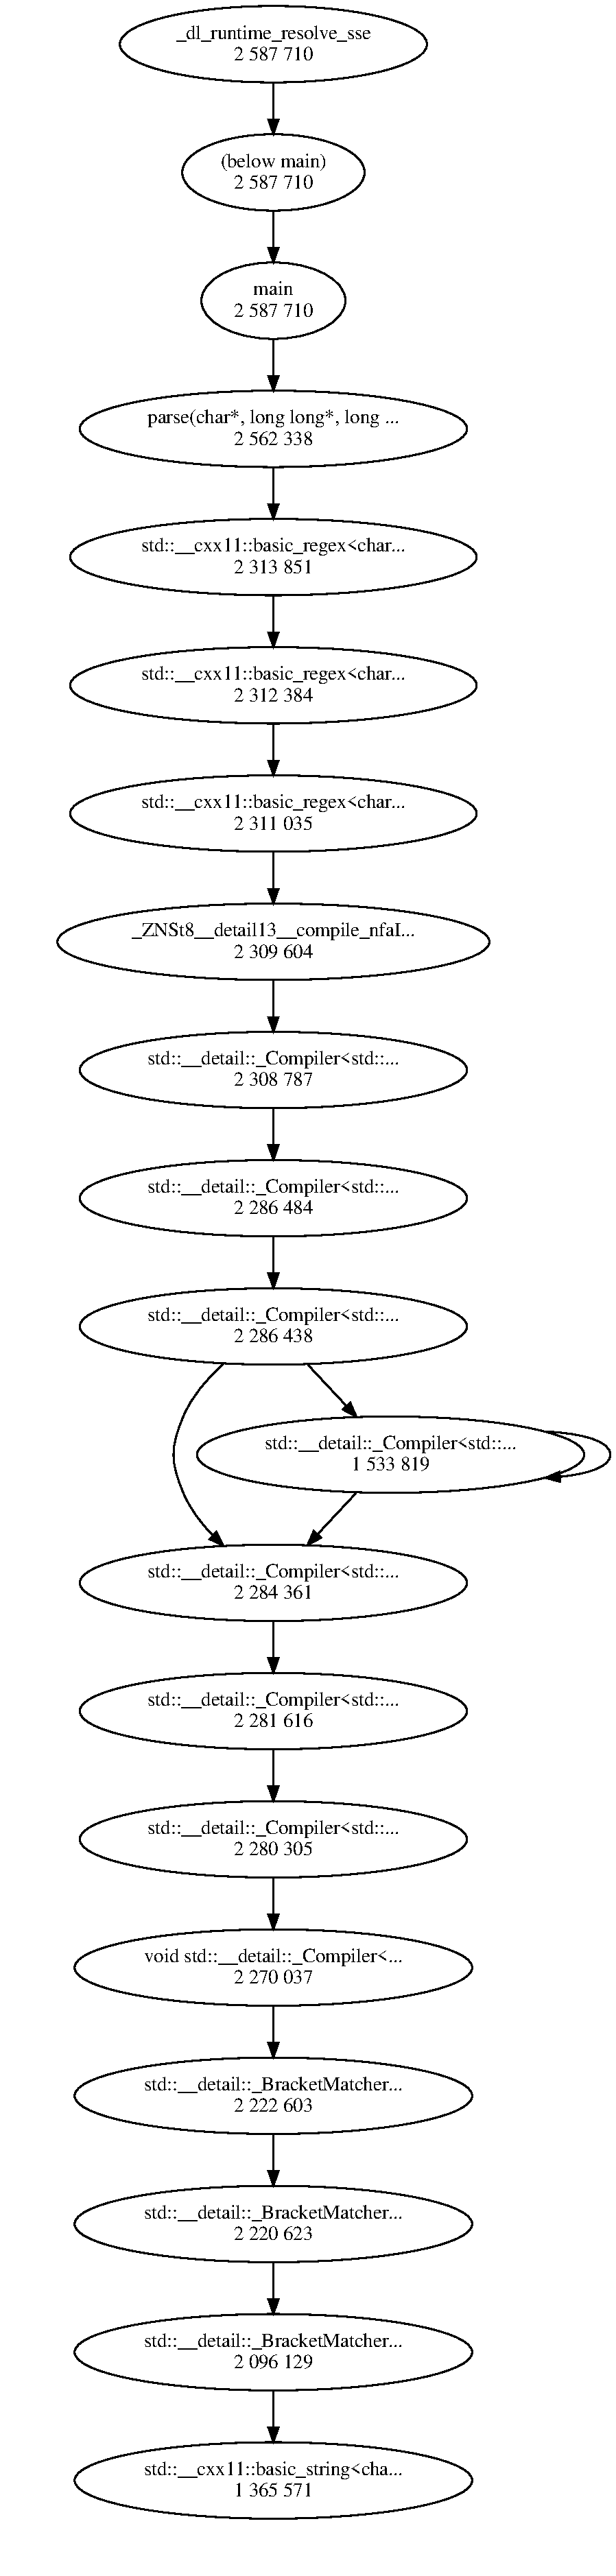
\includegraphics[width=0.33\textwidth]{res/callgraph}
  \caption{Граф вызовов до обфускации}
  \label{fig:myGraph}
\end{center}
\end{figure}

\newpage

Графов вызовов после обфускации (рисунок 2).

\begin{figure}[htp]
\begin{center}
  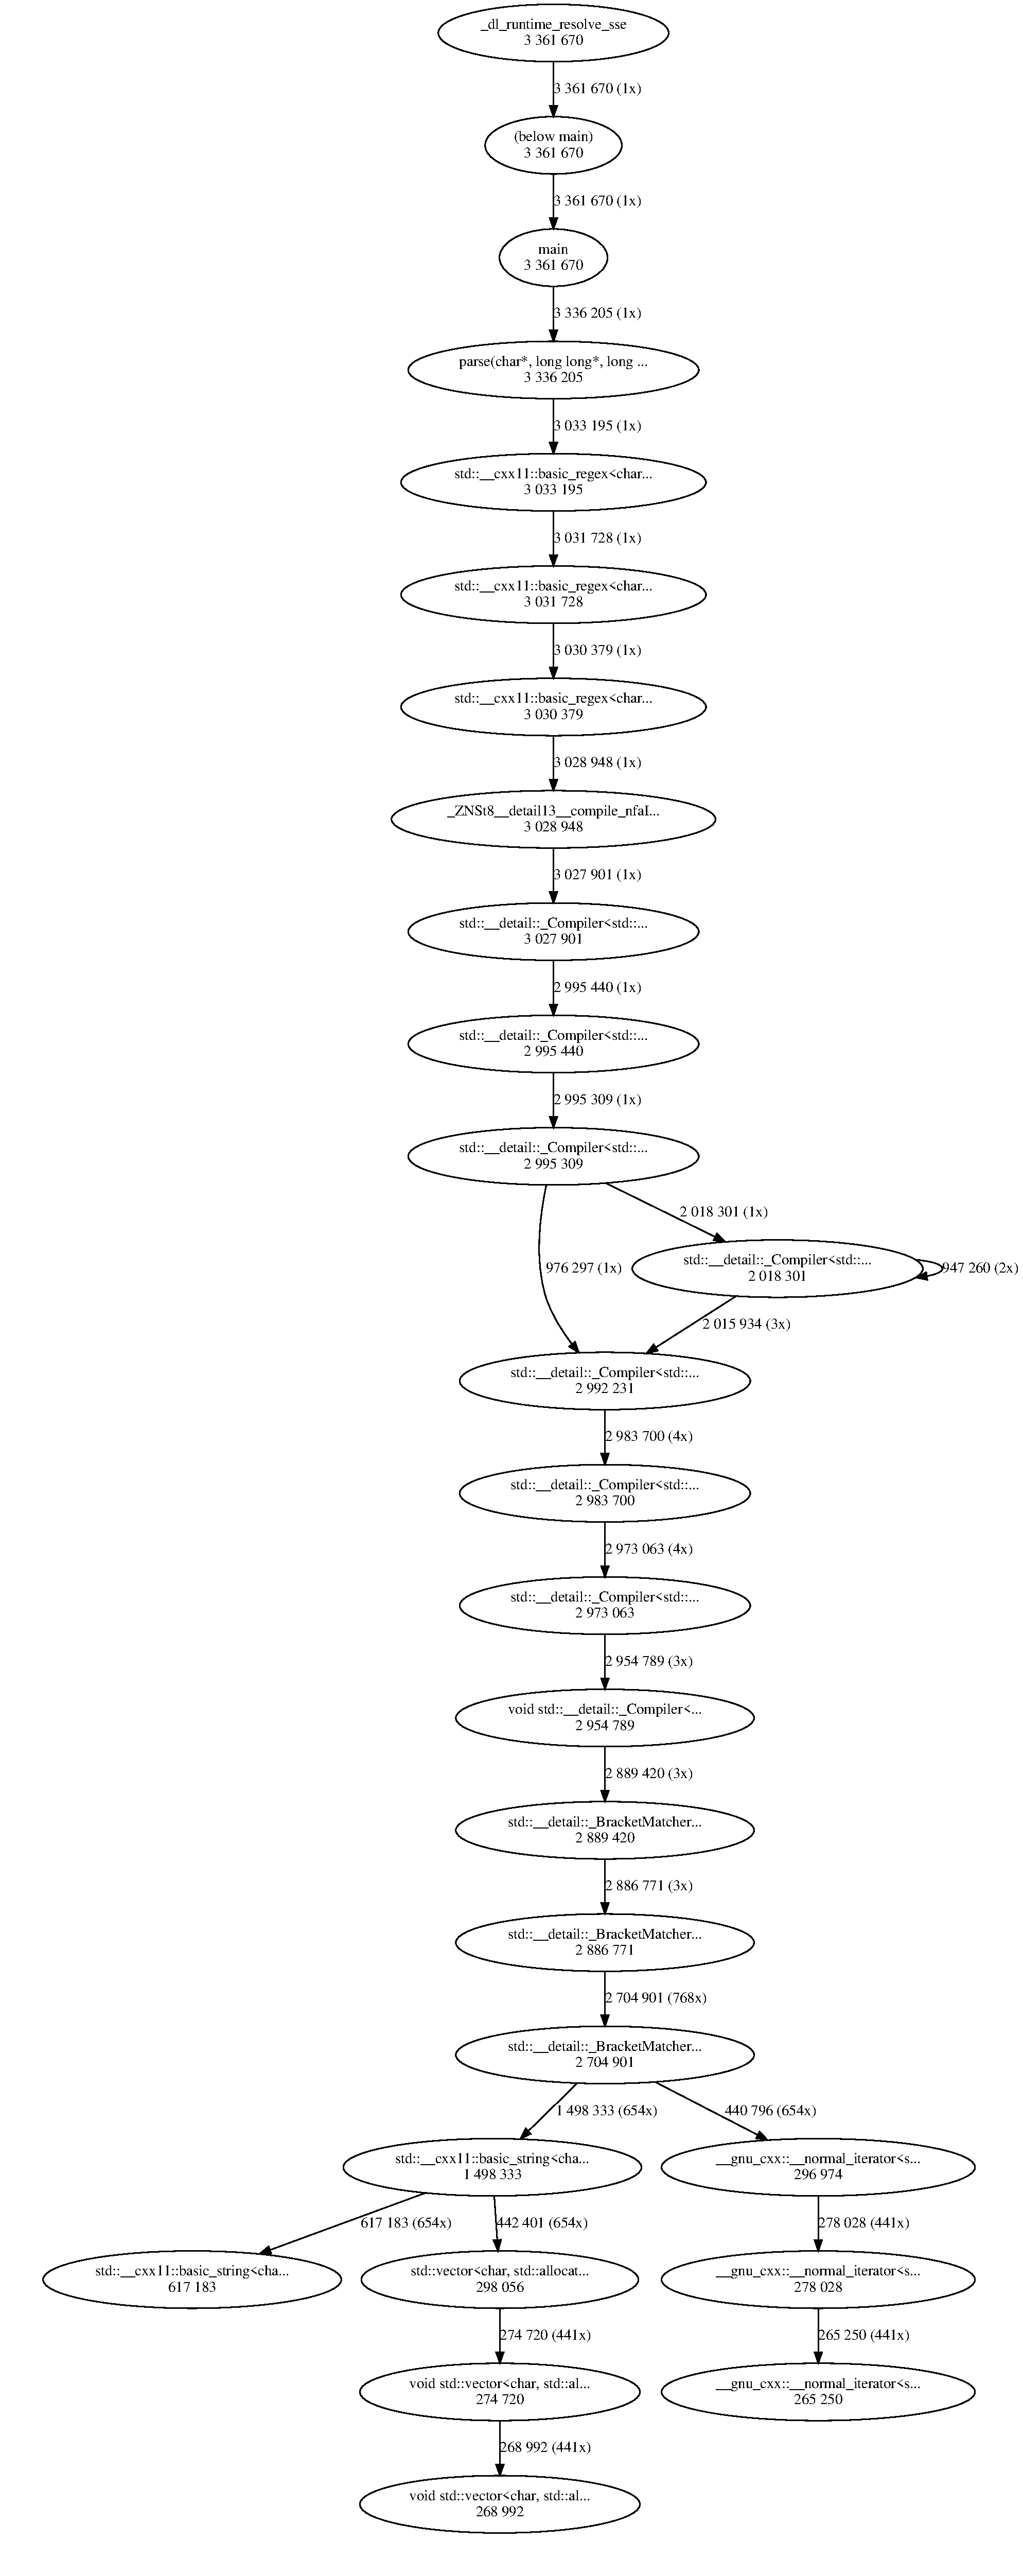
\includegraphics[width=0.41\textwidth]{res/callgraph2}
  \caption{Граф вызовов после обфускации}
  \label{fig:myGraph2}
\end{center}
\end{figure}

Как видно, графы достаточно похожи. Дело в том, что большая часть работы (парсинг строки с использованием регулярных выражений) происходит в стандартной библиотеке C++. Для повышения зашиты можно либо обфусцировать стандартную библиотеку, либо отказаться от её использования и переписать парсинг самостоятельно. Но та часть, которая отвечает за вывод информации, и которая как раз подверглась обфускации, отличается достаточно значительно. % Практическое применение обфускатора

\newpage
%------------------------------------------------
\section*{Заключение}
\addcontentsline{toc}{section}{Заключение}

В данной работе были рассмотрены некоторые системные вызовы, используемые для управления планировщиком при работе с процессами реального времени (POSIX.1b).

В теоретической части было дано описание работы системных вызовов и работы планировщика; по умолчанию все процессы выполняются с интервалос времени равынм 100 мс и приоритетом (nice) 0, который слияет на интервал, позволяя изменять его в диапазоне от 10 мс до 200 мс.

В практической части приведён пример кода, вызывающего изучаемые системные вызовы. Перехват этих вызовов осуществлялся при помощи системной утилиты strace. % Заключение

\newpage
\section*{}
\addcontentsline{toc}{section}{Список литературы}

\begin{thebibliography}{00}

\bibitem{Love} Роберт Лав: «Разработка ядра Linux», Вильямс, 448 стр., 2008, ISBN
5-8459-1085-1, 0-672-32720-1.

\bibitem{Cragon} Harvey G. Cragon: «Computer Architecture and Implementation», Cambridge University Press, 238 pages, 2000, ISBN-10: 521651689.

\bibitem{Rosen} Rami Rosen: «Linux Kernel Networking: Implementation and Theory», Apress, 650 pages, 2014, ISBN-13: 978-1-4302-6196-4.

\bibitem{Realtech} Realtech: RTL8111B, Single-Chip Gigabit LOM Ethernet Controller for PCI Express. Datasheet Rev. 1.4, 02 December 2005, Track ID: JATR-1076-21.

\end{thebibliography} % Источники

%------------------------------------------------------------------------------

\end{document}